\section{Printed Circuit Boards (PCBs)}


\subsection{Allgemeine Informationen}

\begin{minipage}[t]{0.42\columnwidth}
    \subsubsection{Aufgaben PCB}

     \begin{itemize}
        \item Elektrische Verbindung zwischen Bauteilen
        \item Mechanische Befestigung der Bauteile
        \item Wärmeabfuhr
        \item Ev. Abschirmfunktion
        \item Ev. Antennen (kleine Spulen)
     \end{itemize}
\end{minipage}
\hfill
\begin{minipage}[t]{0.56\columnwidth}
    \subsubsection{Testen von PCBs}

    \begin{outline}
        \1 Lot überprüfen
            \2 Automatische Röntgen-Inspektion (AXI)
        \1 Elektrische Überprüfung
            \2 \textbf{In-Circuit-Test} (ICT)
        \1 Bestückung
            \2 Automatische optische Inspektion (AOI)
    \end{outline}
\end{minipage}


\vspace{0.2cm}
\begin{minipage}[t]{0.48\columnwidth}
    \subsubsection{Ausführungen von PCBs}

    \begin{outline}
        \1 Anzahl der Lagen (Layer)
            \2  (4-Lagen als Standard)
        \1 Flex-Leiterplatten
            \2 Stark elatisches Grundmaterial
        \1 Starr-Flex-Leiterplatten
            \2 Kombination aus starr und flexibel
    \end{outline}
\end{minipage}
\hfill
\begin{minipage}[t]{0.48\columnwidth}
    \subsubsection{Gehäuse (Komponenten)}

    \begin{itemize}
        \item THT: through-hole-technology
        \item SMD/SMT: surface mounted device / surface mounted technology
        \item BGA: Ball grid array
        \item CSP: chip scale package
        \item DCA: direct chip attach
     \end{itemize}
\end{minipage}


\subsection{Aufbau von PCBs}

\subsubsection{Lagen-Aufbau}

Ein 4-lagiges PCB ist folgendermassen aufgebaut:

\renewcommand*{\arraystretch}{1}
\begin{center}
    \begin{tabular}{|c|c|c|c|} 
        \toprule
        \textbf{Material}       & \textbf{Lagen}    & \textbf{Typ}      & \textbf{Dicke in mm}      \\
        \midrule
        Cu-Folie                & Lage 1            &                   & 0.018                     \\
        \midrule
        Prepreg                 &                   & Prepreg 7628      & 0.180                     \\
        \midrule
        Prepreg                 &                   & Prepreg 7628      & 0.180                     \\
        \midrule
        Kupfer                  & Lage 2            &                   & 0.035                     \\
        \midrule
        Innenlage               &                   & FR4-Kern          & 0.900                     \\
        \midrule
        Kupfer                  & Lage 3            &                   & 0.035                     \\
        \midrule
        Prepreg                 &                   & Prepreg 7628      & 0.180                     \\
        \midrule
        Prepreg                 &                   & Prepreg 7628      & 0.180                     \\
        \midrule
        Cu-Folie                & Lage 4            &                   & 0.018                     \\
        \midrule
    \end{tabular}
\end{center}


\subsubsection*{Hinweise und Eigenschaften zum Lagen-Aufbau}

\begin{itemize}
    \item Die Gesamt-Dicke eines PCBs ist meist $1.6 \, \milli \meter$ (unabhängig von der Anzahl Layer)
    \item \textbf{PCBs sind immer symmetrisch aufgebaut}
    \item In die Innenlagen sind meist Speisungs-Layer (Flächen mit Speisungen)
    \item Das Basismaterial FR4 besteht aus Epoxidharz und Glasfasergewebe
\end{itemize}


\subsubsection{Durchkontaktierung (Via)}

Die verschiedenen Lagen des PCBs werden mit Vias miteinander verbunden.

\begin{minipage}[c]{0.48\columnwidth}
    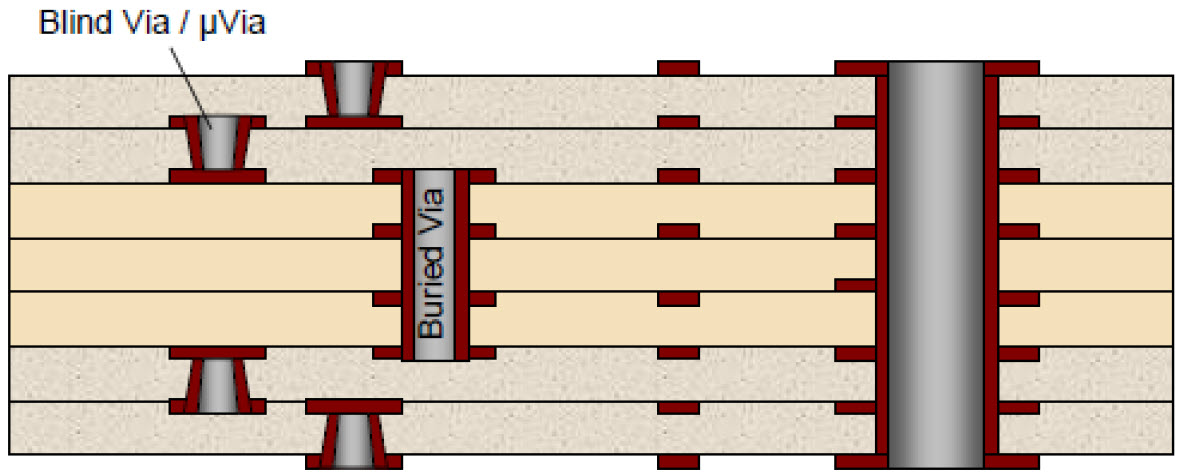
\includegraphics[width=\columnwidth]{images/vias.jpg}
\end{minipage}
\hfill
\begin{minipage}[c]{0.48\columnwidth}
    \begin{outline}
        \1 Buried Via (Vergrabene Durchkontaktierung)
            % \2 In Kernlage liegend; aussen nicht sichtbar
        \1 Blind Via (Sackloch)
            % \2 Auf Innenlage endende Ankontaktierung
        \1 Micro Via
            % \2 An- oder Durchkontaktierung mit Durchmesser $< 200 \, \micro  \meter$
    \end{outline}
\end{minipage}


\subsection{Herstellungsprozess von PCBs}

\begin{outline}
    \1 Vorbereitung und Belichtung der Innenlage (Kern aus FR4)
    \1 Ätzen der Innenlage (Kupfer wird abgeätzt)
    \1 Aussenlage aufbringen und verpressen
    \1 Löcher für Durchkontaktierungen (Vias) bohren
    \1 Durchkontaktieren der Vias (elektrisch verbinden)
    \1 Belichten und Cu-Abscheiden der Aussenlagen
    \1 Aussenlagen ätzen (Leiterbahnen bleiben übrig)
    \1 Lötstoppmaske (solder mask) aufbringen 
    \1 Oberfläche veredeln (Lötpads mit Nickel oder Gold überziehen)
    \1 Bestückungsdruck (silk-screen)
    \1 Fräsungen, Bohrungen (ohne Durchkontaktierung), Tests
\end{outline}


\subsection{Elektrische Eigenschaften von PCBs}

\subsubsection{Widerstand von Leitungen}

\begin{minipage}[t]{0.35\columnwidth}
    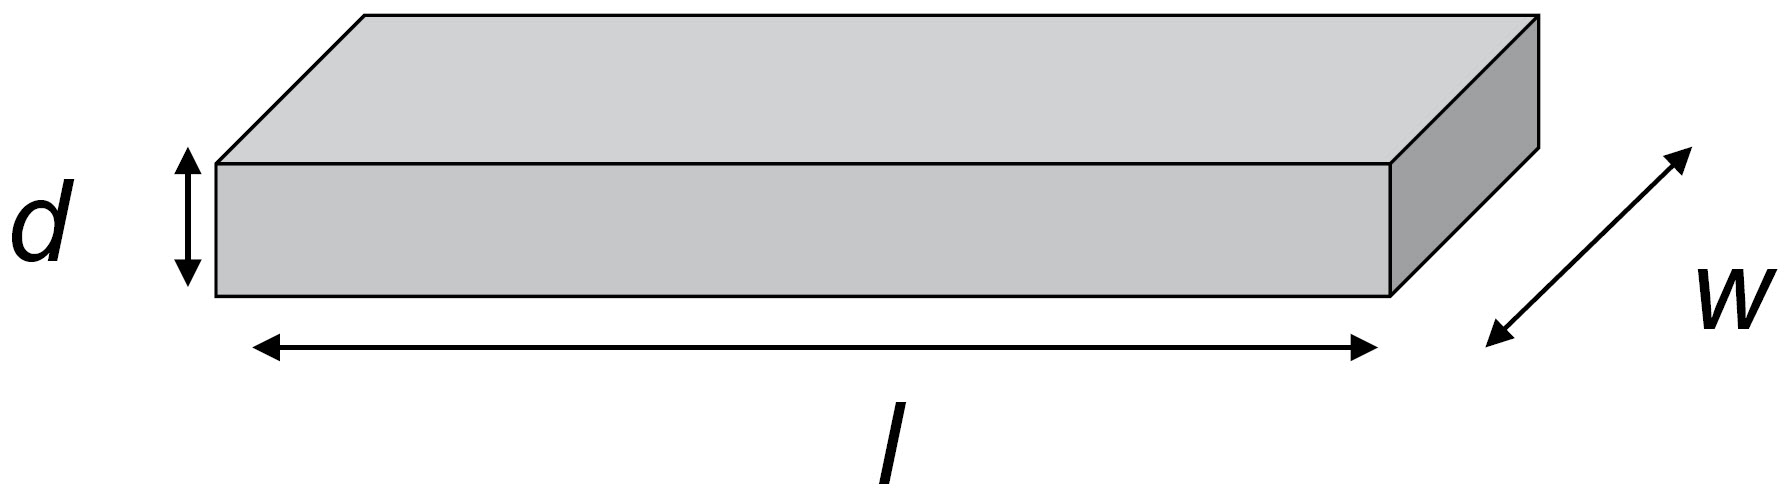
\includegraphics[width=\columnwidth]{images/leitung_widerstand.jpg}
    $$ \boxed{R = \frac{\rho \cdot l}{w \cdot d}} $$
\end{minipage}
\hfill
\begin{minipage}[t]{0.62\columnwidth}
    \begin{tabular}{llc}
        $R$     & Widerstand ($@ \, 20 \, \degree$)         & $[R] = \ohm$ \\
        $\rho$  & spez. Widerstand                          & $[\rho] = \frac{\ohm \milli \meter^2}{\meter}$ \\
        $l$     & Länge des Leiters                         & $[l] = \meter$ \\
        $w$     & Breite des Leiters                        & $[w] = \meter$ \\
        $d$     & Dicke des Leiters ($35 \, \micro \meter$) & $[d] = \meter$ 
    \end{tabular}
\end{minipage}


\subsubsection{Kapazität von Leitungen}

\begin{minipage}[c]{0.28\columnwidth}
    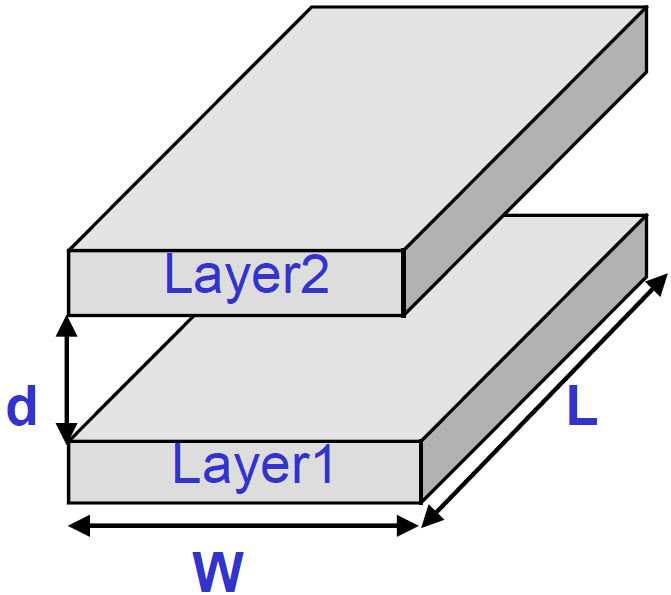
\includegraphics[width=\columnwidth]{images/leitungen_kapazitaet.jpg}
\end{minipage}
\hfill
\begin{minipage}[c]{0.65\columnwidth}
    $ \boxed{C = \frac{\varepsilon_0 \cdot \varepsilon_r \cdot W \cdot L}{d}} $
\end{minipage}

\begin{tabular}{llc}
    $C$             & Kapazität (\textbf{Plattenkondensator!})          & $[C] = \farad$ \\
    $\varepsilon_0$ & elektrische Feldkonstante $8.85 \cdot 10^{-12}$   & $[\varepsilon_0] = \frac{\farad}{\meter}$ \\
    $\varepsilon_r$ & relative Permittivität (FR4: $\varepsilon_r= 4.5$)& $[\varepsilon_r] = 1$ \\
    $A = W \cdot L$ & Fläche der Platten                                & $[A] = \meter$ \\
    $d$             & Abstand zwischen Platten                          & $[d] = \meter$
\end{tabular}


\subsubsection{Induktivität von Leitungen}

\begin{minipage}[c]{0.48\columnwidth}
    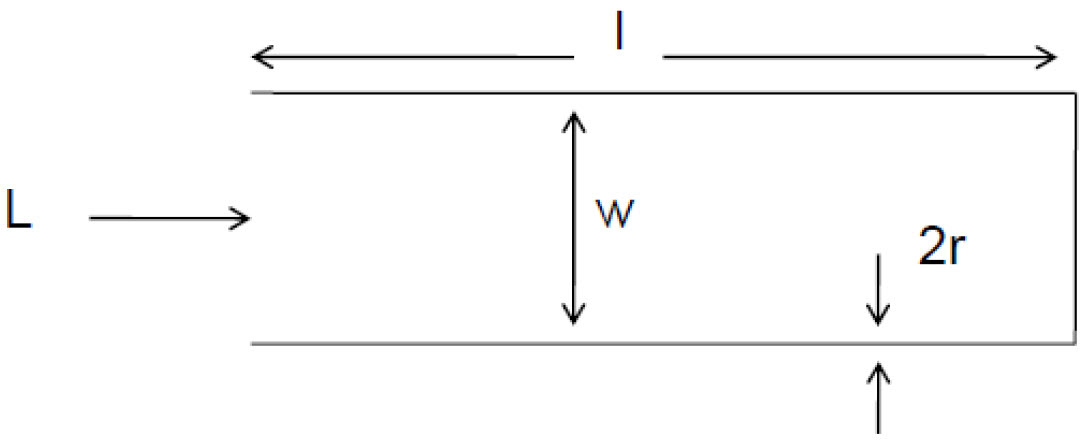
\includegraphics[width=\columnwidth]{images/leitung_induktivitaet.jpg}
\end{minipage}
\hfill
\begin{minipage}[c]{0.48\columnwidth}
    $$ \boxed{ \text{Für } l \gg w \gg r \qquad L = \frac{\mu \cdot l}{\pi} \cdot \ln \Bigg( \frac{w}{r} \Bigg) } $$
\end{minipage}


\subsection{Signalfluss auf dem PCB}

\begin{minipage}[c]{0.48\columnwidth}
    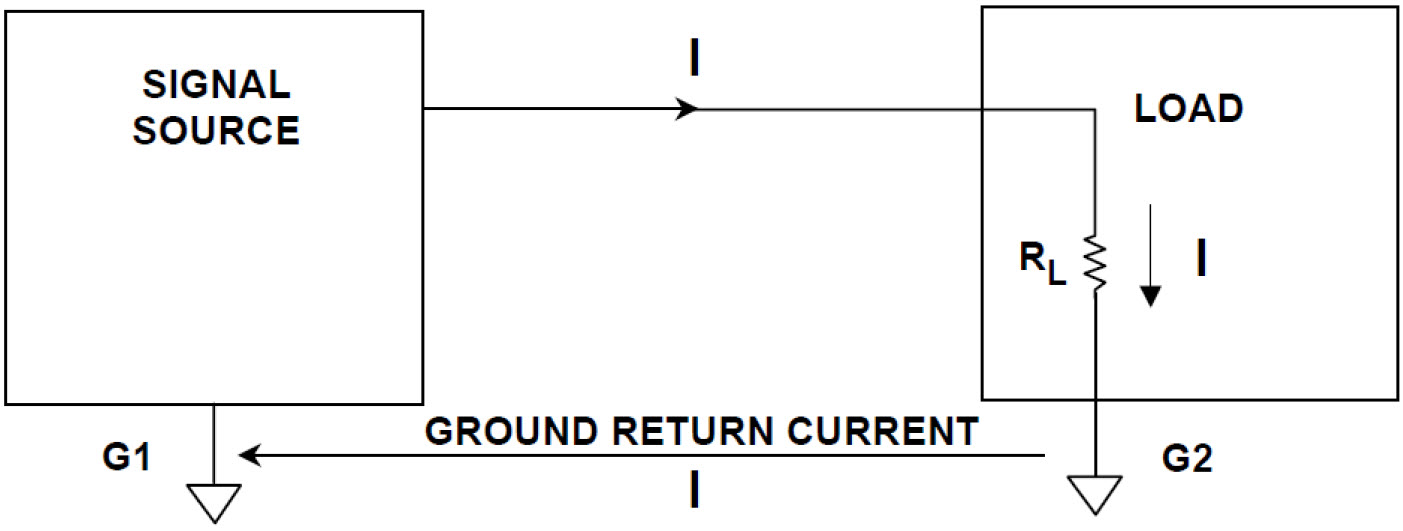
\includegraphics[width=\columnwidth]{images/signalfluss_pcb.jpg}
\end{minipage}
\hfill
\begin{minipage}[c]{0.48\columnwidth}
    \begin{outline}
        \1 \textbf{Strom fliesst immer zurück!}
            \2 Leitung oder \textbf{ground planes}
        \1 Rückstrom nimmt Weg des geringsten Widerstands (geringste Impedanz)
    \end{outline}
\end{minipage}

